\header{
    \section{Billy le Bordelais} \label{billy-le-bordelais}
    %
    
    \insertComment{Chanson de Joe Dassin (1970) paroles de Pierre Delanoë.}{}
}

\enluminure{4}{\href{https://www.youtube.com/watch?v=YFFTwYm_nuA}{D}}{ès} sa naissance
\\C'est fou quand on y pense
\\Avec violence
\\Il refusa le lait
\\Que sa nourrice
\\Une fille sans malice
\\Venue de Suisse
\\Gentiment lui donnait
\\\\Car le bon vin de Saint Emilion
\\Ça vous donne un coeur de lion
\\A condition d'en mettre dans les biberons
\\C'était un bébé ni beau ni laid
\\Avec de petits mollets
\\Mais déjà le monde l'appelait
\\Billy le bordelais (qui ?)
\\Billy le bordelais
\begin{figure}[h!]
\centering
   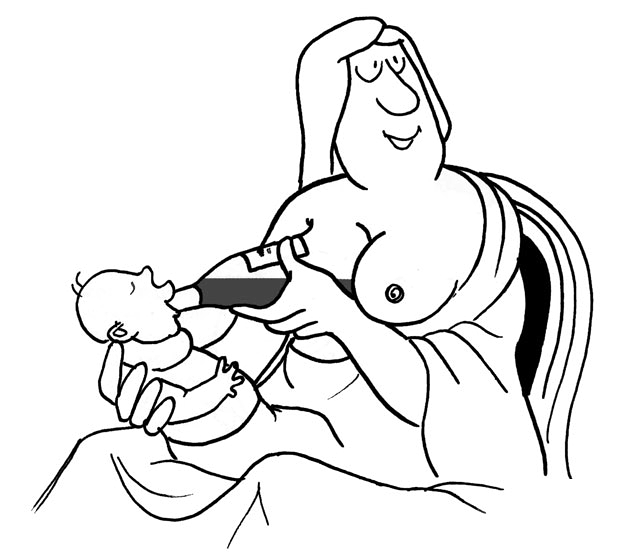
\includegraphics[width=0.7\textwidth]{images/Billy.png}
 \end{figure}
\breakpage
\\\\L'enfant terrible
\\Avait l'horreur morbide
\\De ce liquide
\\Que l'on appelle de l'eau
\\La plus mauvaise
\\Étant la flotte anglaise
\\Billy à l'aise
\\Nous vengea de Waterloo
\\\\Car le bon vin de Saint Emilion
\\Ca vous donne un coeur de lion
\\Ah qu'il était content le Napoléon
\\Il dit à Billy : "Toi, tu me plais
\\Pour tout ce que tu as fait
\\Moi, je te donne la Bourgogne"
\\Billy le bordelais (qui ça ?)
\\Billy le bordelais
\\\\De la Castille
\\A la mer des Antilles
\\Toutes les filles
\\De Billy raffolaient
\\Des messalines
\\Des reines et des tsarines
\\Des ursulines
\\Tout le monde y passait
\\\\Car le bon vin de Saint Emilion
\\Ça vous donne un coeur de lion
\\Pour trousser les jupons et les cotillons
\\Avec tous les enfants qu'il a fait
\\Je me demande si tu n'es
\\Ou si je ne suis pas bâtard de
\\Billy le bordelais (qui ?)
\\Billy le bordelais
\\\\Messieurs, mesdames
\\Voici la fin du drame
\\L'appel aux armes
\\Laissez vos larmes couler
\\Billy l'unique
\\Billy le magnifique
\\C'est historique
\\Est mort assassiné
\\\\Car le bon vin de Saint Emilion
\\Ca vous donne un coeur de lion
\\Mais l'ennemi guettait le pauvre garcon
\\On lui a glissé dedans son verre
\\De l'eau à dose mortelle
\\Il est mort dans un dernier glouglou
\\Billy le bordelou (qui ?)
\\Billly le bordeli (non !)
\\Billy le bordelon (le vrai !)
\\Billy le bordelais
\\\\\textbf{Envoi : }
\\Prince, Duc, Marquis
\\Ou Monsieur de Bordeaux
\\Ton sang est fait de vin
\\Bien plus qu'il ne l'est d'eau
\\Aussi je te dédie cette histoire attachante
\\Espérant que demain, toi aussi, tu la chantes !

\vspace{1cm}
\begin{figure}[h!]
\centering
   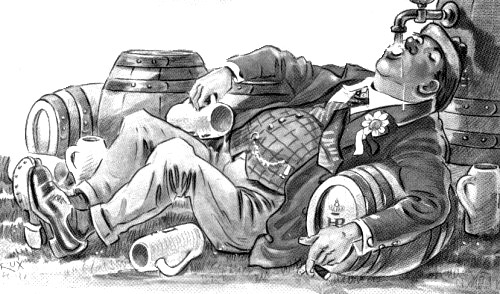
\includegraphics[width=0.9\textwidth]{images/bourguignone.jpg}
 \end{figure}

\breakpage